%\vspace*{-.4cm}
\section{Introduction}
\label{sec:intro}
%\vspace*{-.2cm}

Even if more flexible and often more efficient approaches to the
Virtual Machine Placement Problem (VMPP) have been developed,
most of the popular Cloud Computing (CC) system
management \cite{cloudstack,opennebula,openstack}, \aka
Infrastructure-as-a-Service toolkits~\cite{moreno:2012}, continue to
rely on elementary Virtual Machine (VM) placement policies that
prevent them from maximizing the usage of CC resources while
guaranteeing VM resource requirements as defined by Service Level
Agreements (SLAs).
% %% THE TEXT BELOW COMES FROM ISPA'13
% %%%%%%%
Typically, a batch scheduling approach is used: VMs are allocated
according to user requests for resource reservations and tied to
the nodes where they were deployed until their destruction. Besides
the fact that users often overestimate their resource requirements,
such static policies are definitely not optimal for CC providers,
since the effective resource requirements of each operated VM may
significantly vary during its lifetime.

An important impediment to the adoption of more advanced strategies
such as consolidation, load balancing and other SLA-ensuring
algorithms that have been deeply investigated by the research community
%\cite{feller:ccgrid12,Hermenier:2009:ECM:1508293.1508300,5715067,quesnel:cpe2012,5328077,5935254}
%is related to the experimental
% REMOVE: 5328077 can be removed if need be
\cite{feller:ccgrid12,Hermenier:2009:ECM:1508293.1508300,quesnel:cpe2012,5328077,5935254} is related to the experimental
processes that have been used to validate them: most VMPP proposals have
been evaluated either by leveraging ad-hoc simulators or small \textit
{in-vivo} experiments. These evaluation environments are not accurate and not
representative enough to (i) ensure their correctness on real
platforms and (ii) perform fair comparisons between them.
%
% %
% \begin{figure}[ht]
% \vspace*{-.2cm}
% \begin{center}
%         \subcapcentertrue
%         \subfigure[Scheduling steps]{
%         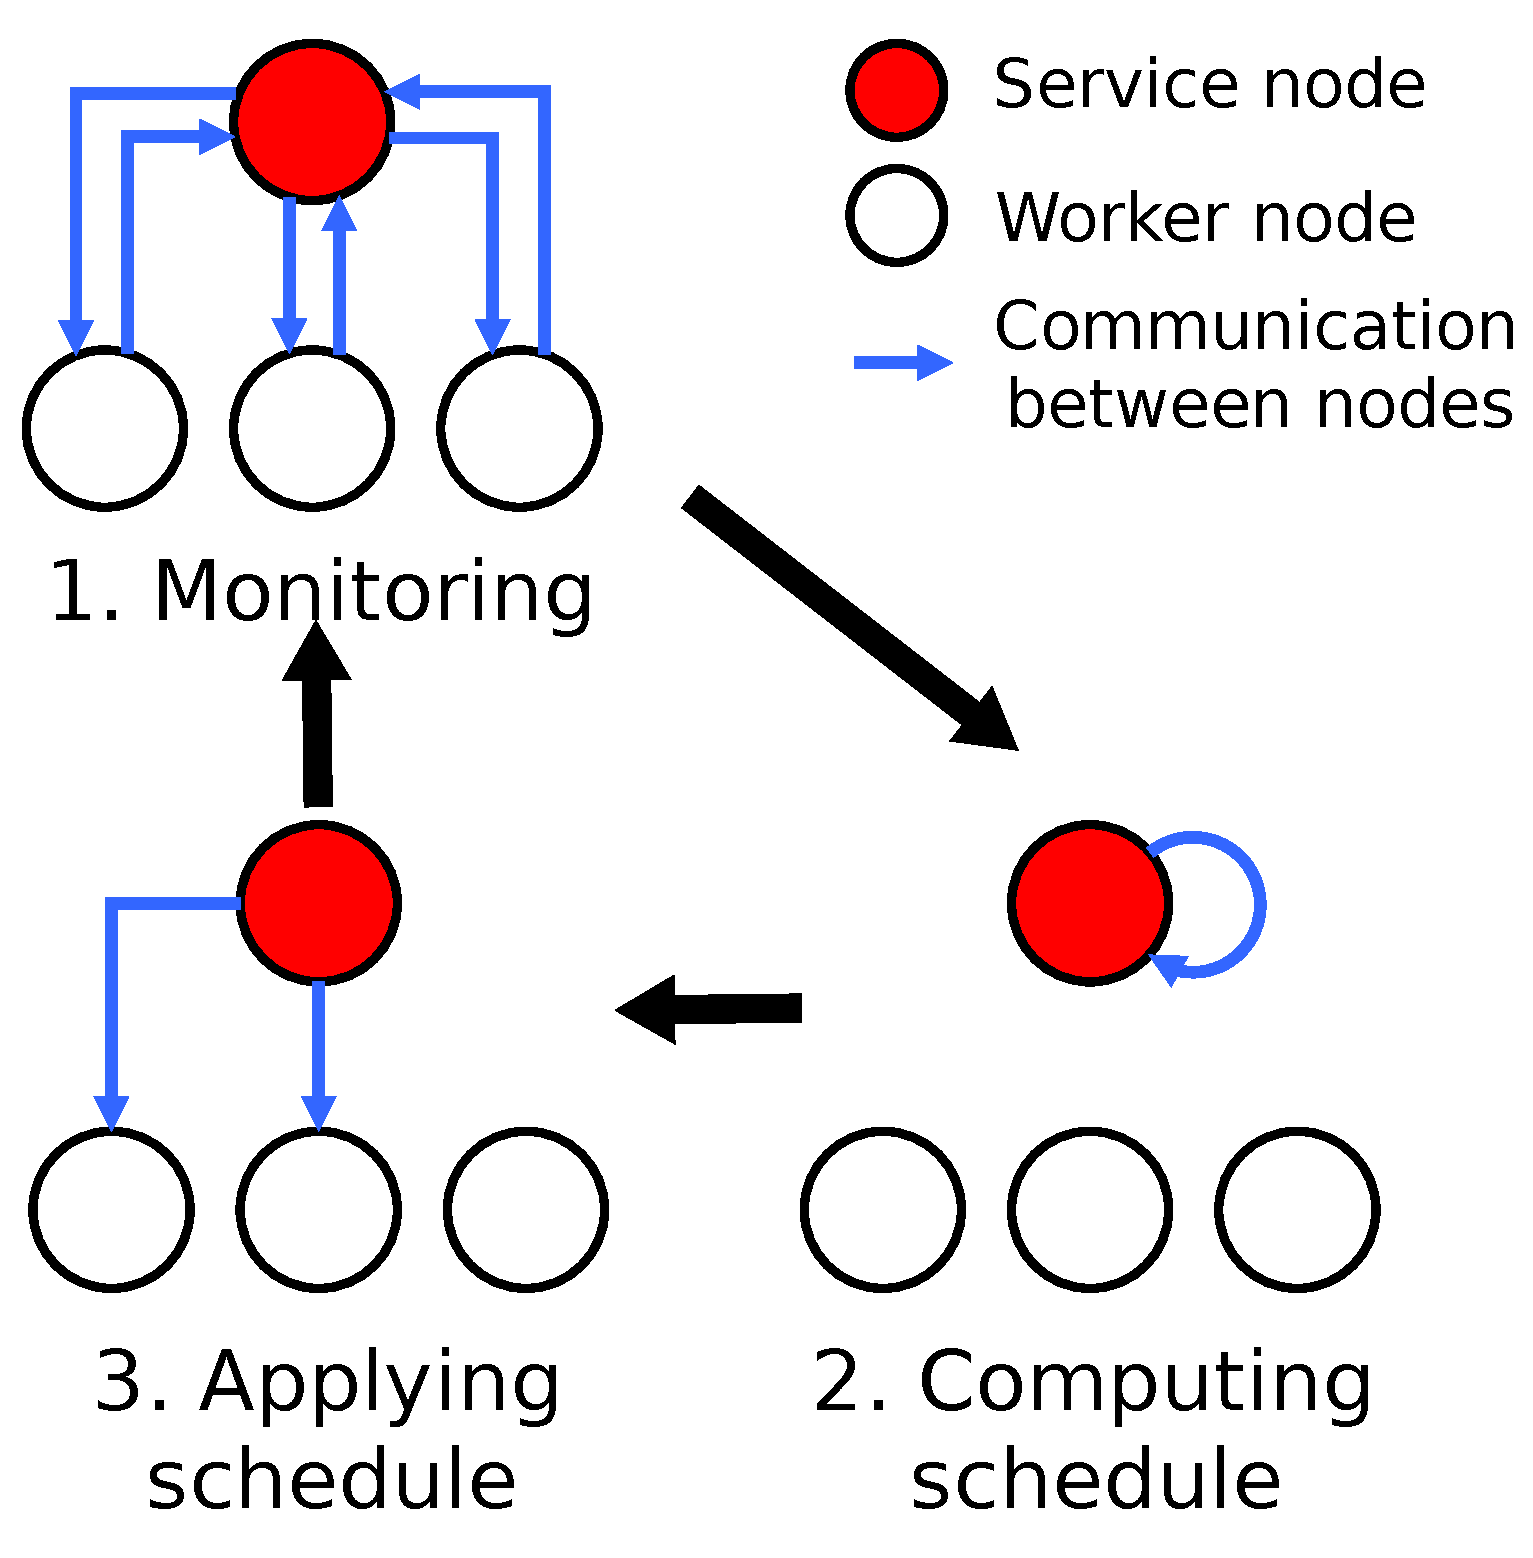
\includegraphics[width=.45\linewidth]{figures/scheduling_steps.pdf}
%         \label{fig:scheduling_steps}}
%         \subfigure[Workload fluctuations during scheduling]{
%         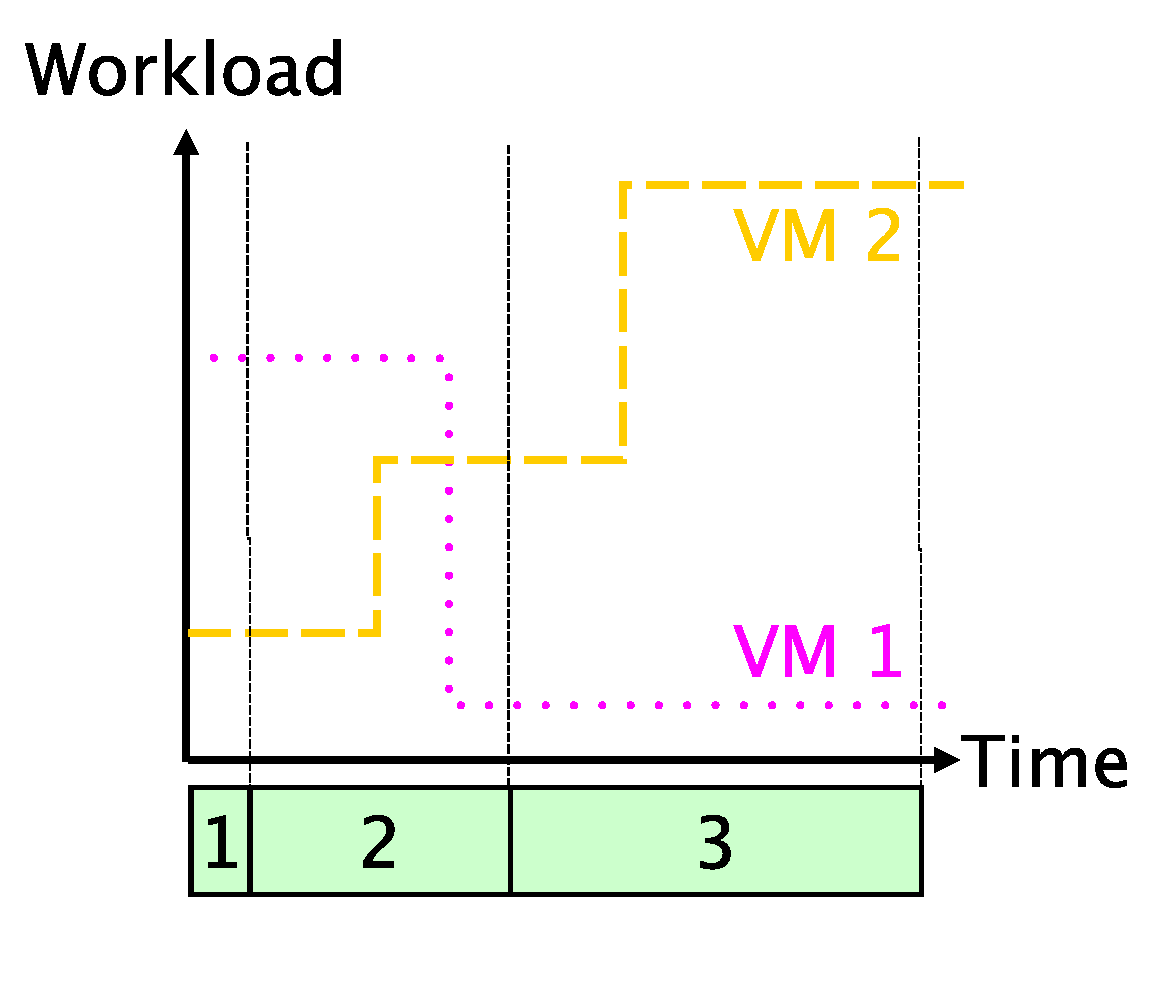
\includegraphics[width=.45\linewidth]{figures/workload_fluctuations2.pdf}
%         \label{fig:workload_fluctuations}}
% \vspace*{-.2cm}
% \caption{VM scheduling in a master/worker architecture}
% \end{center}
% \label{fig:scheduling}
% \vspace*{-.2cm}
% \end{figure}
% %
% \MS[AL]{Must we keep the fig.: the arguments of complexity and time
%   requirements are already made in the remainder of the intro. If we
%   keep it, the discussion should be simplified.}
% Each VMPP mechanism is a complex system that can face
% important side-effects during each of its stages: Monitoring the
% resources usages, computing the schedule and applying the
% reconfiguration (see Figure \ref{fig:scheduling_steps}).
% %
% %
% As an example, a single master architecture can lead, \textit{a priori} to
% important drawbacks. First, during the computation and the application
% of a schedule, a single master cannot take into account new VM
% requirement violations. Second, the time needed to apply a new
% schedule can be particularly important: The longer the reconfiguration
% process, the higher the risk that the schedule may be outdated, due to
% the workload fluctuations, when it is eventually applied (see Figure
% \ref{fig:workload_fluctuations}). Finally, a single master node can
% lead to well-known fault-tolerance issues: A group of VMs may be
% temporarily isolated from the master node in case of a network
% disconnection or if the master node crashes.
% %
Implementing each proposal and evaluating it on representative
testbeds in terms of scalability, reliability and varying workload
changes would definitely be the most rigorous way to observe and
propose appropriate solutions for CC production infrastructures.
% and compare  with existing proposals.
However, \textit{in-vivo} (\ie real-world) experiments, if they can be
executed at all, are always expensive and tedious to perform (for
recent reference see~\cite{barker:pitfalls}).
% They may even be counterproductive if the observed behaviors are clearly
%different from the expected ones.

In this article, we propose \vmps, a dedicated simulation framework to
perform in-depth investigations of VM placement algorithms and compare
them in a fair way. To cope with real conditions such as the
increasing scale of modern data centers and the workloads dynamicity
that are specific to the CC paradigm, notably its elasticity
capacity, \vmps allows users to study large-scale scenarios
%that take into account server crashes and
that involve thousands of VMs,
each executing a specific workload that evolves during the
simulation lifetime.
%
To illustrate the relevance of \vmps, we have implemented and analyzed
three VMPP approaches:
Entropy~\cite{Hermenier:2009:ECM:1508293.1508300},
Snooze~\cite{feller:ccgrid12}, and DVMS~\cite{quesnel:cpe2012}.
Besides being well-known from the literature, we chose
these three systems as they are built on three different software
architecture approaches: Entropy relies on a centralized model, Snooze
on a hierarchical one and DVMS on a fully distributed one.
Results returned by \vmps enable us to discuss the
scalability and reactivity (\ie the time to solve
resource violations, \aka SLA violation) criterions of each strategy.
In particular, this study reveals the importance of the duraction of
the reconfiguration phase (\ie the step where VMs are relocated throughout the infrastructure) in
comparison to the computation one (\ie the step where the scheduler try to solve the VMPP).
%
%Built on top of the \sg toolkit~\cite{casanova:hal-01017319},
We believe that \vmps  will be beneficial to a large number of researchers in the field
of CC as it enables them to quickly validate
the trends of a new proposal, allowing \textit{in vivo} experiments to be
restricted to VMPP mechanisms that have the potential to handle CC
production infrastructures.

The rest of the article is
organized as follow.
%Section~\ref{sec:vmpp} highlights the importance of the scalability, reliability and reactivity criterions for the VM
%Placement Problem.
Section~\ref{sec:sg} gives an overview of the \sg
framework on which our proposal is built. \ref{sec:injector}
introduces \vmps and discusses its general functioning. The three
algorithms implemented as use-cases are presented in
Section~\ref{sec:vm-schedulers} and evaluated in
Section~\ref{sec:experiments}. Section~\ref{sec:related} and
Section~\ref{sec:conclusion} present, respectively, related work as
well as a conclusion and future work.
